%17/10 - Óscar
\chapter{Acceso programático a bases de datos biomédicas}
\section{Introducción}
En este bloque queremos acceder mediante los programas a las bases de datos biomédicas y poder interactuar con ellas. Las bases de datos biomédicas no están especialmente bien diseñadas; es decir, hay que aprender hacer peticiones desde el protocolo HTTP. Un protocolo es un lenguaje en el que interactúan las dos partes: queremos pedirle a la base de datos unas entradas que nos devuelve y poder utilizarlas. Nos tendremos que crear un protocolo intermedio para poder interactuar con la base de datos. Como esto puede ser un lío, se diseñaron las API REST. Un API es application programming interface, es decir, un protocolo o una manera de interactuar con otra parte en un formato concreto. REST tiene que ver con el protocolo HTTP de base. El protocolo HTTP se utiliza para navegar por internet. Todas las aplicaciones exponen un API REST, lo que quiere decir que hay unas ciertas órdenes o funciones que se pueden llamar para que la aplicación haga cosas. Hay una serie de endpoints, que son cada una de las funciones que se van a llamar: un endpoint para buscar un organismo concreto, para descargar una cierta secuencia, etc. 

Hay varias maneras de acceder a bases de datos en línea (nivel de abstracción o automatización ascendente):
\begin{itemize}
\item \textbf{Copiar la base de datos de manera local}: procesos manuales, pero se queda rápidamente desactualizada. Se puede descargar un fichero de un servicio web en Linux mediante \texttt{wget url/base/de/datos/fichero.txt}
\item \textbf{Rellenar formularios}: todavía no se ha actualizado el acceso mediante API, pero se puede escribir en Python un programa que rellene el formulario como si fuera un humano para acceder a los datos cambiando los valores de los parámetros. En general, la sintaxis de una URL es la siguiente:\\
scheme:[//host]path[?query][\#fragment]\\
siendo scheme HTTP o HTTPS cuando el protocolo está cifrado y es seguro (la s viene de secure), host el servidor que contiene la base de datos que se quiere acceder, el path la ruta para llegar a una parte del servidor (como si fueran carpetas), la interrogración el marcador de los argumentos (las queries en formato nombre=valor\&nombre2=valor2). Así, lo que queremos hacer con Python es codificar los distintos argumentos para poder acceder a varias entradas de forma automática. Por ejemplo, en el formulario tipo \href{https://www.ebi.ac.uk/Tools/dbfetch/dbfetch?db=ena\_sequence\&id=J00231\&style=raw}{https://www.ebi.ac.uk/Tools/dbfetch/dbfetch?db=ena\_sequence\&id=J00231\&style=raw}, en lugar de rellenar el formulario varias veces, queremos cambiar el valor de los distintos argumentos (id=J00231, id=J00232, id=J00233, db=afdb, etc.). 
\item Peticiones HTTP directa: esto se puede conseguir mediante la librería \texttt{requests} en Python.
\item Uso específico de API: Hay algunos servicios que proporcionan APIs de los servidores para poder utilizarlos desde Python. Esto se conoce como APIs de alto nivel o SDKs. Esta es la mejor manera, ya que es más cómoda y más fácil de utilizar, pero no está disponible en todas las bases de datos.
\end{itemize} 

\subsection{Acceso programático}
Hay varias librerías disponibles en Python para automatizar el acceso y procesado de las URL:
\begin{itemize}
\item \texttt{urllib}: acceso de bajo nivel, más adecuado para programación de red.
\item \texttt{requests}
\end{itemize}

La librería requests tiene el comando \texttt{get}, que es el método HTTP más común. 
\begin{lstlisting}[language=Python]
import requests
url = "https://www.ebi.ac.uk/Tools/dbfetch/dbfetch?db=ena_sequence&id=J00231&style=raw"
response = requests.get(url)
print(response.text)
\end{lstlisting}

En el método \texttt{get} de requests se puede utilizar el argumento \texttt{params} para pasar los distintos argumentos. Este argumento debe ser un diccionario con los distintos parámetros:
\begin{lstlisting}[language=Python]
import requests

ebi_url = 'https://www.ebi.ac.uk/Tools/dbfetch/dbfetch'

response = requests.get(ebi_url,
    params={'db': 'ena_sequence', 'id':'J00231' , 'style':'raw'})

print(response.text)
\end{lstlisting}

\section{JSON}
Hay distintas formas de poder representar un fichero:
\begin{itemize}
\item Texto plano
\item HTML (HyperText Markup Language)
\item XML (eXtensible Markup Language)
\item JSON (JavaScript Object Notation)
\end{itemize}

La notación JSON es similar a la de los diccionarios en Python conceptualmente: las claves son strings y los valores pueden ser strings, números, listas o incluso diccionarios. Técnicamente es una forma de estructurar la información (figura \ref{fig:json}) en formato ASCII. 

\begin{figure}[htbp]
\centering
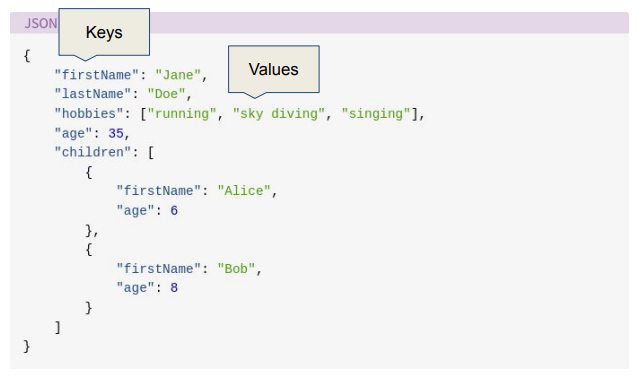
\includegraphics[width = 0.7\textwidth]{figs/json.png}
\caption{Ejemplo de un fichero JSON que describe a una persona. Las llaves representan estructuras y los corchetes listas.}
\label{fig:json}
\end{figure}

Python cuenta con una librería llamada \texttt{json}.
\begin{lstlisting}[language=Python]
import json

json_data =  '{"name":"John", "age":30, "city":"New York"}'

print(json_data)
\end{lstlisting}

%\section{Protocolo HTTP}


%\section{API REST}


